\documentclass[../main/report.tex]{subfiles}
\begin{document}
\chapter{Discussion}

\subfile{../discussion/design_process.tex}

\section{PCB}
Split project schematics into several connected docs for the sake of modularity. Find some overarching hardware requirements and from there, related application notes and hardware considerations. Then some components and footprints that fit...ish with these docs.
Finally place components and route the wires between them digitally and order the PCB and components


\section{USB data input}
In the initial design, a USB connector was introduced to receive data from a host PC. 
But during the implementation phase, it was discovered to be unnecessary.
For the graphical demo, there was no need for input data from host PC. 
The MCU was able to run the program independently.


\section{VGA-port}
The PCB was designed with two VGA headers, one for the FPGA and one for the MCU. \todo{Maybe add picture showing the headers.}
Looking back, it was redundant to support two VGA ports.
An alternative solution is having one VGA port with exposed headers.
With exposed headers from the MCU and the FPGA as well, one could change which one the VGA port is connected to by jumpers like \ref{fig:vga-solution}.
By removing one of the VGA ports, the size of the PCB could have been reduced, or used for other components. 


\begin{figure}[H]
    \centering
    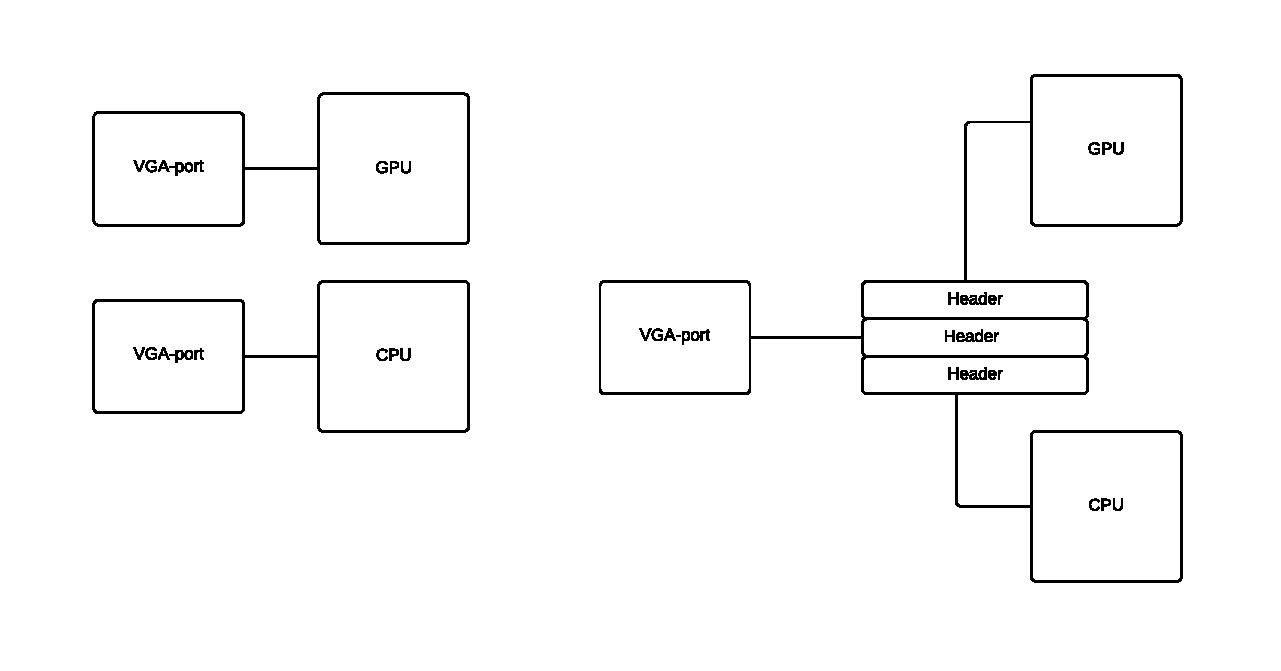
\includegraphics[width=\textwidth]{../discussion/assets/vga-solution.pdf}
    \label{fig:vga-solution}
    \caption{On the left: The current setup on our PCB. On the right: The alternative solution.}
\end{figure}



\subfile{../discussion/energy_efficiency.tex}

\section{"Jaktstart"}

Not everyone can start at the same time

\section{Redundancy design choices or w/e}
What did we end up needing?
What could we have used, that we didn't think of.

\section{Does the computer make sense?}
Is the design sane?
Were we idiots?
Have we seen the light?

\section{Can we even saturate the memory bus?}
Do you even SRAM?
Or is memory the big bottleneck

\section{SRAM bottleneck}
HDMI vs. the GPU?
Will the HDMI be fine with always being second in line?

\end{document}
